% !TeX program = xelatex

% UI-Thesis v1.0

% این قالب بر اساس فرمت پایان‌نامه‌ها و رساله‌های تحصیلات تکمیلی دانشگاه اصفهان تهیه شده است.
% علیرضا روحی-دانشجوی دکتری گروه مهندسی نرم افزار دانشگاه اصفهان
% 1395
% rouhi.ir@gmail.com
% توصیه می‌شود که از توزیع تک‌لایو (TexLive2015) به بعد استفاده شود:
% http://tug.org/texlive/acquire-iso.html

% موفق باشید.
% با تشکر از امین فخاری که قالب اصلی این پایان نامه را برای دانشگاه صنعتی اصفهان تهیه نموده اند.
% 1395
% a101.fakhari@gmail.com
% -----------------------------------------------------------------------------------

% نکات:

% برای آن‌که پردازش فایل و مشاهده خروجی در هنگام نوشتن پایان‌نامه آسان‌تر و سریع‌تر انجام شود، انجام موارد زیر توصیه می گردد:
% الف) فصل‌ها و بخش‌هایی که در حال نوشتن آن‌ها نیستید را غیر فعال کنید. به‌عنوان مثال، در این قالب، این دستورات را می‌توان در صورت عدم نیاز با اضافه کردن % به طور موقت غیرفعال کرد:
% \MakeTitlePage
% \MakeFarsiSignaturePage
% % !TEX root = ../ui-thesis.tex
% !TeX program = xelatex

\clearpage
\thispagestyle{empty}
\newgeometry{left=3.5cm,right=3.5cm,top=7cm}

{\BNazaninScaleOne
{\fontsize{20pt}{0}\selectfont \bfseries
\noindent
% عنوان تشکر و قدردانی---------------------------------------------------------
سپاس‌گزاری
% ؛---------------------------------------------------------
}}
\vspace{0.5cm}

{\BNazaninScaleOne
{\fontsize{12pt}{0.9cm}\selectfont % ‌B Nazanin 13
\noindent
% متن تشکر و قدردانی---------------------------------------------------------
خدایا تو را شاکرم به خاطر امروزم که به من عطا فرمودی...






% ؛---------------------------------------------------------
}}

\restoregeometry
% \MakeCopyRightPage
% % !TEX root = ../ui-thesis.tex
% !TeX program = xelatex

\clearpage
\thispagestyle{empty}
\newgeometry{left=3.5cm,right=3.5cm,top=7cm}

{\BNazaninScaleOne
{\fontsize{20pt}{0}\selectfont \bfseries
\noindent
% تقدیم اثر---------------------------------------------------------
تقدیم به
\\[1cm]
\hspace*{1cm}
خودم
% ؛---------------------------------------------------------
}}
		
\restoregeometry
% \MakeTableOfContents
% \MakeListOfFigures
% \MakeListOfTables
% \MakeFarsiAbstract
% \input{Chapters/Chapter#}
% \MakeAppendices
% % !TEX root = ../ui-thesis.tex
% !TeX program = xelatex

\section{جزئیات معادله‌ها}
لورم ایپسوم متن ساختگی با تولید سادگی نامفهوم از صنعت چاپ و با استفاده از طراحان گرافیک است. چاپگرها و متون بلکه روزنامه و مجله در ستون و سطرآنچنان که لازم است و برای شرایط فعلی تکنولوژی مورد نیاز و کاربردهای متنوع با هدف بهبود ابزارهای کاربردی می باشد. کتابهای زیادی در شصت و سه درصد گذشته، حال و آینده شناخت فراوان جامعه و متخصصان را می طلبد تا با نرم افزارها شناخت بیشتری را برای طراحان رایانه ای علی الخصوص طراحان خلاقی و فرهنگ پیشرو در زبان فارسی ایجاد کرد. در این صورت می توان امید داشت که تمام و دشواری موجود در ارائه راهکارها و شرایط سخت تایپ به پایان رسد وزمان مورد نیاز شامل حروفچینی دستاوردهای اصلی و جوابگوی سوالات پیوسته اهل دنیای موجود طراحی اساسا مورد استفاده قرار گیرد.

لورم ایپسوم متن ساختگی با تولید سادگی نامفهوم از صنعت چاپ و با استفاده از طراحان گرافیک است. چاپگرها و متون بلکه روزنامه و مجله در ستون و سطرآنچنان که لازم است و برای شرایط فعلی تکنولوژی مورد نیاز و کاربردهای متنوع با هدف بهبود ابزارهای کاربردی می باشد. کتابهای زیادی در شصت و سه درصد گذشته، حال و آینده شناخت فراوان جامعه و متخصصان را می طلبد تا با نرم افزارها شناخت بیشتری را برای طراحان رایانه ای علی الخصوص طراحان خلاقی و فرهنگ پیشرو در زبان فارسی ایجاد کرد. در این صورت می توان امید داشت که تمام و دشواری موجود در ارائه راهکارها و شرایط سخت تایپ به پایان رسد وزمان مورد نیاز شامل حروفچینی دستاوردهای اصلی و جوابگوی سوالات پیوسته اهل دنیای موجود طراحی اساسا مورد استفاده قرار گیرد.
\begin{equation}
p\left( r \right) = {C_k}\frac{N}{{\pi {a^2}}}{\left[{1 - {{\left( {\frac{r}{a}} \right)}^k}} \right]^{\frac{1}{k}}}
\label{Eq:Pressure1}
\end{equation}
است.

\newpage
\section{اثبات روابط ریاضی}
نلورم ایپسوم متن ساختگی با تولید سادگی نامفهوم از صنعت چاپ و با استفاده از طراحان گرافیک است. چاپگرها و متون بلکه روزنامه و مجله در ستون و سطرآنچنان که لازم است و برای شرایط فعلی تکنولوژی مورد نیاز و کاربردهای متنوع با هدف بهبود ابزارهای کاربردی می باشد. کتابهای زیادی در شصت و سه درصد گذشته، حال و آینده شناخت فراوان جامعه و متخصصان را می طلبد تا با نرم افزارها شناخت بیشتری را برای طراحان رایانه ای علی الخصوص طراحان خلاقی و فرهنگ پیشرو در زبان فارسی ایجاد کرد. در این صورت می توان امید داشت که تمام و دشواری موجود در ارائه راهکارها و شرایط سخت تایپ به پایان رسد وزمان مورد نیاز شامل حروفچینی دستاوردهای اصلی و جوابگوی سوالات پیوسته اهل دنیای موجود طراحی اساسا مورد استفاده قرار گیرد. (شکل~%
\ref{Fig:World1})
لورم ایپسوم متن ساختگی با تولید سادگی نامفهوم از صنعت چاپ و با استفاده از طراحان گرافیک است. چاپگرها و متون بلکه روزنامه و مجله در ستون و سطرآنچنان که لازم است و برای شرایط فعلی تکنولوژی مورد نیاز و کاربردهای متنوع با هدف بهبود ابزارهای کاربردی می باشد. کتابهای زیادی در شصت و سه درصد گذشته، حال و آینده شناخت فراوان جامعه و متخصصان را می طلبد تا با نرم افزارها شناخت بیشتری را برای طراحان رایانه ای علی الخصوص طراحان خلاقی و فرهنگ پیشرو در زبان فارسی ایجاد کرد. در این صورت می توان امید داشت که تمام و دشواری موجود در ارائه راهکارها و شرایط سخت تایپ به پایان رسد وزمان مورد نیاز شامل حروفچینی دستاوردهای اصلی و جوابگوی سوالات پیوسته اهل دنیای موجود طراحی اساسا مورد استفاده قرار گیرد.
\begin{figure}[!htb]
\centering
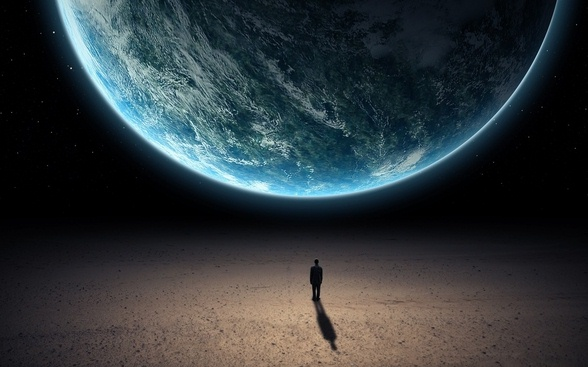
\includegraphics[scale=0.4]{Figures/World.jpg}
\caption{تصویر مفهومی}
\label{Fig:World1}
\end{figure}

لورم ایپسوم متن ساختگی با تولید سادگی نامفهوم از صنعت چاپ و با استفاده از طراحان گرافیک است. چاپگرها و متون بلکه روزنامه و مجله در ستون و سطرآنچنان که لازم است و برای شرایط فعلی تکنولوژی مورد نیاز و کاربردهای متنوع با هدف بهبود ابزارهای کاربردی می باشد. کتابهای زیادی در شصت و سه درصد گذشته، حال و آینده شناخت فراوان جامعه و متخصصان را می طلبد تا با نرم افزارها شناخت بیشتری را برای طراحان رایانه ای علی الخصوص طراحان خلاقی و فرهنگ پیشرو در زبان فارسی ایجاد کرد. در این صورت می توان امید داشت که تمام و دشواری موجود در ارائه راهکارها و شرایط سخت تایپ به پایان رسد وزمان مورد نیاز شامل حروفچینی دستاوردهای اصلی و جوابگوی سوالات پیوسته اهل دنیای موجود طراحی اساسا مورد استفاده قرار گیرد.
% \MakeEnglishAbstract
% \MakeEnglishSignaturePage
% ب) از گزینه draft برای فراخوانی کلاس استفاده کنید. یعنی
% \documentclass[a4paper,fleqn,13pt,twoside,draft]{book}
% این گزینه حالت چرکنویس را ایفا می‌کند و بر روی بسته‌های مختلف اثرهای متفاوتی دارد. به‌عنوان مثال: به جای شکل، تنها چهارچوب آن نمایش داده شود، لینک‌های hyperref غیر فعال گردد، فایل‌های خارجی را در بسته listings اضافه نمی‌کند و ... و همه این موارد سبب کاهش زمان اجرا و حجم فایل می‌شود.

% در صورتی که میخواهید به سطر بعد بروید اما نمیخواهید بین دو کلمه‌ای که نوشتید فاصله بیفتد کافی است در انتهای خط اول  (بدون فاصله) کاراکتر % را اضافه کنید. با این عمل، لاتک خط فاصله ایجاد شده در اثر تغییر سطر را به عنوان توضیح اضافه یا کامنت در نظر میگیرد و در خروجی اعمال نمی‌کند.

% توصیه می‌شود از شکل‌های برداری با فرمت PDF استفاده شود. این کار علاوه بر افزایش کیفیت رسال/پایان‌نامه/گزارش، باعث کاهش حجم شکل‌ها (و در نتیجه  کاهش حجم فایل نهایی) و همچنین کاهش زمان پردازش می‌شود.

% در این قالب سعی شده است که از تمامی بخش‌های موجود در پایان‌نامه‌ها نمونه‌ای آورده شود.

\documentclass[a4paper,fleqn,11pt,oneside]{book}
\usepackage{tikz}
\usetikzlibrary{arrows,shapes}
\usepackage{tabulary}
\usepackage{Settings/UI-Thesis}
\usepackage{acronym}
\usepackage{multirow}

%-----------------------------
% دستورهای مورد نیاز را در این قسمت اضافه نمایید:
% Cross-reference commands.
\newtheorem{thm}{Theorem}[chapter]
\newtheorem{asmp}{Theorem}[chapter]
\theoremstyle{definition}
\newtheorem{definition}[thm]{تعریف}
\newtheorem{assumption}[asmp]{فرض}
\newtheorem{example}{مثال}[chapter]

\newcommand{\xs}[1]{بخش~\ref{#1}}
\newcommand{\xc}[1]{فصل~\ref{#1}}
\newcommand{\xp}[1]{صفحه~\pageref{#1}}
\newcommand{\xf}[1]{شکل~\ref{#1}}
\newcommand{\xt}[1]{جدول~\ref{#1}}
\newcommand{\xa}[1]{پیوست~\ref{#1}}
\newcommand{\xd}[1]{تعریف~\ref{#1}}
\newcommand{\xr}[1]{قانون~\ref{#1}}
\newcommand{\xra}[1]{R~\ref{#1}}
\newcommand{\xl}[1]{کد~\ref{#1}}
\newcommand{\xal}[1]{الگوریتم~\ref{#1}}
\newcommand{\xe}[1]{معادله~\eqref{#1}}
\newcommand{\xex}[1]{مثال~\ref{#1}}
\newcommand{\xeq}[1]{رابطه~\eqref{#1}}

\newcommand{\mylr}[1]{\texorpdfstring{\lr{#1}}{#1}}
\eqenvironment{نکات}{itemize}
\eqenvironment{تعریف}{definition}
\eqcommand{مورد}{item}

%%%%%%%%%%%%%%%%%%%%%%%%%%%%%%%%%%%%%%%%%%%%%%%%%%%%%%%%%%%%%%



%\DeclareMathSizes{9}{9}{9}{9}

\lstset{escapeinside={/*@}{@*/}}
%\definecolor{codebackground}{rgb}{0.95,0.95,0.95}
\definecolor{codebackground}{RGB}{255,255,255}
\definecolor{commentcolor}{RGB}{77,153,153}
\definecolor{keywordcolor}{RGB}{153,77,153}
\lstset{backgroundcolor=\color{codebackground}}

\lstset{
  captionpos=b,
  numberstyle=\tiny,
  %basicstyle=\ttfamily\footnotesize,
  %basicstyle=\setLTR\thefootnotesize\ttfamily,
  basicstyle=\setLTR\bfseries\fontsize{8.5pt}{0}\selectfont\ttfamily,
  columns=flexible,
  tabsize=2,
  numbers=none, %left,
  nolol=true,
  keywordstyle=\color{keywordcolor},
  commentstyle=\color{commentcolor},
  stringstyle=\color{blue},
  captiondirection=RTL,
  upquote=true,
}

\def\lstlistingname{کد}

%\input{listings/EOLFormat}
%-----------------------------

\begin{document}



\pagestyle{plain}
\pagenumbering{harfi}
%\setcounter{page}{2}

% ░░░░░░░▒▒▒▒▒▒▓▓▓▓ In the Name of Allah ▓▓▓▓▒▒▒▒▒▒░░░░░░░
\clearpage
\thispagestyle{empty}
\newgeometry{left=3.5cm, right=3.5cm, top=3.5cm, bottom=3.5cm}
\begin{figure}
  \centering

\includegraphics[width = \linewidth]{Settings/Allah.png}
\end{figure}
% ░░░░░░░▒▒▒▒▒▒▓▓▓▓ Title Page ▓▓▓▓▒▒▒▒▒▒░░░░░░░
\DepartmentFa{دانشکده مهندسی کامپیوتر}
\GroupFa{گروه مهندسی نرم‌افزار}
\ThesisTypeFa{پروژه درس روش پژوهش و ارائه} % Or \ThesisTypeFa{پایان‌نامه} Or \ThesisTypeFa{پیشنهادیه پایان‌نامه}
\DegreeFa{کارشناسی} % Or \DegreeFa{کارشناسی ارشد}
\FieldFa{مهندسی کامپیوتر}
\BranchFa{ هوش مصنوعی}   % This is نام گرایش
\YourFullnameFa{ سهیل سلیمی}
\FirstSupervisorFa{زهرا زجاجی}
\YearFa{ دی 1402}
\TitleFa{ استفاده از کانتینر ها برای اجرای سریع و محلی\\ [0.4cm] مدل های زبانی بزرگ}

% اگر عنوان رساله طولانی بود، در دو خط به صورت نشان داده شده تقسیم شود.
%\TitleFa{قسمت اول عنوان \\ [0.4cm] قسمت دوم عنوان}

\MakeTitlePage


% ░░░░░░░▒▒▒▒▒▒▓▓▓▓ Dedication ▓▓▓▓▒▒▒▒▒▒░░░░░░░
% !TEX root = ../ui-thesis.tex
% !TeX program = xelatex

\clearpage
\thispagestyle{empty}
\newgeometry{left=3.5cm,right=3.5cm,top=7cm}

{\BNazaninScaleOne
{\fontsize{20pt}{0}\selectfont \bfseries
\noindent
% تقدیم اثر---------------------------------------------------------
تقدیم به
\\[1cm]
\hspace*{1cm}
خودم
% ؛---------------------------------------------------------
}}
		
\restoregeometry

% ░░░░░░░▒▒▒▒▒▒▓▓▓▓ Abstract - Farsi ▓▓▓▓▒▒▒▒▒▒░░░░░░░
% !TEX root = ../ui-thesis.tex
% !TeX program = xelatex


\AbstractFa{
  مدل های زبانی بزرگ \LTRfootnote{Large language model} مدل هایی هستند که با استفاده از تکنیک های یادگیری عمیق بر روی داده های متنی بزرگ آموزش دیده اند و قادر به تولید متن های شبیه به انسان و انجام وظایف مختلف بر اساس ورودی ارائه شده هستند. این مدل ها می توانند برای تولید محتوای خلاق، ترجمه زبان ها، پاسخ به سوالات و انجام وظایف دیگر مورد استفاده قرار گیرند. اما اجرای این مدل ها در محیط های واقعی با چالش هایی مانند نیاز به منابع محاسباتی زیاد، حفظ حریم خصوصی و امنیت داده ها، و مسئولیت اخلاقی مواجه است. در این مقاله، ما یک روش برای استفاده از کانتینر ها برای اجرای سریع و محلی ﻣﺪﻝ ﻫﺎﻱ ﺯﺑﺎﻧﻲ ﺑﺰﺭگ را ارائه می دهیم. کانتینر ها امکان ایجاد و اجرای محیط های نرم افزاری مستقل و قابل حمل را فراهم می کنند. ما نشان می دهیم که چگونه می توان با استفاده از کانتینر ها، مدل های زبانی را بدون نیاز به یک سرویس ابری، بر روی دستگاه های محلی اجرا کرد. ما مزایا و چالش های این روش را بررسی می کنیم و چندین مورد کاربردی را نشان می دهیم. ما نتایج آزمایش های خود را بر روی چندین مدل زبانی معروف و چندین وظیفه زبانی ارائه می دهیم و نشان می دهیم که این روش می تواند کارایی و دقت بالایی را حفظ کند. ما همچنین چندین جهت برای کارهای آینده در این زمینه پیشنهاد می دهیم.  
}

\KeywordsFa{
 1- کانتینر ها و مدل های زبانی بزرگ
 2- اجرای محلی و سریع مدل های زبانی
 3- بهینه سازی و امنیت مدل های زبانی
 4- مورد کاربردی مدل های زبانی بزرگ
}
\MakeFarsiAbstract

% ░░░░░░░▒▒▒▒▒▒▓▓▓▓ Table of Contents/Figures/Tables ▓▓▓▓▒▒▒▒▒▒░░░░░░░
\setcounter{page}{0}

\MakeTableOfContents
\MakeListOfFigures
\MakeListOfTables

% ----------------------------------------------------------------------------
\clearpage
\pagestyle{myheadings}
\pagenumbering{arabic}
\setcounter{page}{1}

% ░░░░░░░▒▒▒▒▒▒▓▓▓▓ Chapters ▓▓▓▓▒▒▒▒▒▒░░░░░░░
\clearpage
\baselineskip=0.9cm
\setcounter{footnote}{0}

% !TEX root = ../ui-thesis.tex
% !TeX program = xelatex
\chapter{مقدمه}
\section{پیش‌گفتار}

مدل های زبانی بزرگ \LTRfootnote{Large language model} \cite{min2023recent} در سال های اخیر توانایی شگفت انگیزی در وظایف پردازش زبان طبیعی و فراتر از آن نشان داده اند. این موفقیت مدل های زبانی بزرگ  ها منجر به ورود تعداد زیادی از پژوهش های علمی در این زمینه شده است. این پژوهش ها موضوعات متنوعی را شامل می شوند، از جمله نوآوری های معماری، راهبردهای بهتر آموزش، بهبود طول متن، تنظیم دقیق، مدل های زبانی بزرگ  های چند حالته، رباتیک، مجموعه داده ها، معیارهای ارزیابی، کارایی و بیشتر. با توجه به توسعه سریع روش ها و پیشرفت های مداوم در پژوهش مدل های زبانی بزرگ  ها، درک تصویر کلی از پیشرفت ها در این راستا بسیار چالش برانگیز شده است.

در این مقاله، ما به بررسی چالش ها و راه حل های مربوط به اجرای سریع و محلی مدل های زبانی بزرگ  ها می پردازیم. ما نشان می دهیم که چگونه می توان با استفاده از کانتینر ها، یک روش مدیریت بسته بندی و انتشار نرم افزار، مدل های زبانی بزرگ  ها را بر روی رایانه های شخصی یا سرورهای خود اجرا کرد. این به معنای این است که نیازی به تکیه بر یک سرویس ابری برای استفاده از آنها نیست، که می تواند چندین مزیت داشته باشد، از جمله: حفظ حریم خصوصی و امنیت داده ها: وقتی یک مدل های زبانی بزرگ  محلی را اجرا می کنید، داده های شما هرگز از دستگاه شما خارج نمی شود. این می تواند برای داده های حساس، مانند سوابق بهداشتی یا داده های مالی، مهم باشد. در دسترس بودن آفلاین: مدل های زبانی بزرگ  های محلی می توانند آفلاین استفاده شوند، که به این معنی است که شما می توانید از آنها حتی اگر اتصال اینترنت نداشته باشید، استفاده کنید. این می تواند برای کار بر روی پروژه های در مناطق دور افتاده یا برای برنامه هایی که نیاز به در دسترس بودن همیشگی دارند، مفید باشد. سفارشی سازی: مدل های زبانی بزرگ  های محلی می توانند برای وظایف یا حوزه های خاص تنظیم دقیق شوند. این می تواند آنها را دقیق تر و کارآمدتر برای وظایفی که شما نیاز دارید انجام دهند، کند. مدل های زبانی بزرگ  ها می توانند بر روی انواع پلتفرم های سخت افزاری، از جمله واحد پردازش مرکزی \LTRfootnote{CPU} ها و واحد پردازش گرافیکی \LTRfootnote{GPU} ها اجرا شوند. با این حال، مهم است توجه داشته باشید که مدل های زبانی بزرگ  های محلی می توانند بسیار هزینه بر برای اجرا باشند، بنابراین شما ممکن است به یک رایانه قدرتمند برای استفاده از آنها به طور موثر نیاز داشته باشید. برای اجرای یک مدل های زبانی بزرگ  محلی، شما باید نرم افزار لازم را نصب کنید و فایل های مدل را دانلود کنید. پس از انجام این کار، شما می توانید مدل را شروع کنید و از آن برای تولید متن، ترجمه زبان ها، پاسخ به سوالات و انجام وظایف دیگر استفاده کنید. 
% !TEX root = ../ui-thesis.tex
% !TeX program = xelatex

\chapter{مطالب اصلی}
\section{ادبیات موضوع}
\subsection{کانتینر ها}

کانتینر سازی یک روش مدیریت بسته بندی و انتشار نرم افزار است که به شکل مجازی برنامه های کاربردی را برای استقرار، بسته بندی و ایزوله می کند\cite{hayut1981containerization}. کانتینرها از هسته سیستم عامل استفاده می کنند تا برنامه های کاربردی را از سخت افزار و سیستم عامل میزبان جدا کنند. این باعث می شود که برنامه ها قابل انتقال، سبک و سریع باشند.


کانتینر ها مفهومی هستند که به برنامه نویسان امکان می دهند تا برنامه های خود را به صورت مستقل و قابل انتقال بین محیط های مختلف اجرا کنند. کانتینر ها(شکل \ref{Fig:container}) را می توان با کانتینر کشی تشبیه کرد. کانتینر کشی یک روش حمل و نقل است که در آن کالاهای مختلف در جعبه های استاندارد قرار می گیرند و با استفاده از وسایل نقلیه مختلف مثل کشتی، قطار، کامیون یا هواپیما حمل می شوند. کانتینر های برنامه نویسی هم مثل جعبه های حمل و نقل، برنامه های مختلف را در خود جای می دهند و با استفاده از سیستم عامل های مختلف مثل لینوکس، ویندوز، مک یا اندروید اجرا می شوند. کانتینر ها از برنامه ها جدا هستند و فقط به منابع لازم برای اجرای آن دسترسی دارند. این باعث می شود که برنامه ها سبک تر، سریع تر و امن تر باشند. کانتینر ها همچنین به برنامه نویسان امکان می دهند تا برنامه های خود را به راحتی به روز رسانی، تست، اشکال زدایی و توزیع کنند.

\begin{figure}[!htb]
  \centering
  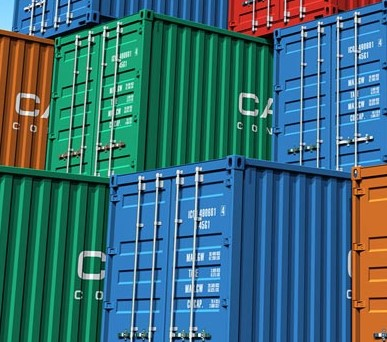
\includegraphics[scale=1]{Figures/container.jpg}
  \caption{نظم دهی کانتینر های به وسایل برای حمل}
  \label{Fig:container}
  \end{figure}

  \begin{example}[کاربرد داکر]
    \centering
    \label{example:docker}
 فرض کنید شما یک برنامه وب نوشته شده با پایتون دارید که از چندین کتابخانه و پکیج استفاده می کند. برای اجرای این برنامه، شما نیاز دارید که سیستم عامل، پایتون و تمام وابستگی های آن را نصب کنید. اگر شما بخواهید برنامه خود را به یک سرور دیگر منتقل کنید، شما باید همین کار را در آن سرور نیز تکرار کنید. این فرآیند زمان بر، خطا خیز و ناکارآمد است.

\end{example}

با استفاده از کانتینر ها، شما می توانید برنامه خود را به همراه تمام وابستگی های آن در یک فایل قابل حمل قرار دهید. این فایل را می توان به عنوان یک تصویر \LTRfootnote{image} کانتینر نامید. سپس شما می توانید با استفاده از یک نرم افزار مدیریت کانتینر، مثل داکر \LTRfootnote{Docker}، این تصویر را در هر سرور یا محصول دلخواه خود اجرا کنید. داکر مسئول این است که تصویر را به یک فرآیند در حال اجرا \LTRfootnote{container} تبدیل کند و با سطح مناسب از جداسازی و امنیت، آن را در سیستم عامل میزبان قرار دهد. به این ترتیب، شما نگران نصب و پیکربندی وابستگی های برنامه خود در هر محصول نخواهید بود.


مدیریت کانتینر یک فرآیند است که به ایجاد، اجرا، مانیتورینگ، توقف و حذف کانتینرها می پردازد3. برای مدیریت کانتینرها، نیاز به ابزارهایی است که به عنوان ارکستراسیون کانتینر شناخته می شوند. این ابزارها به مدیریت کانتینرهای متعدد بر روی یک یا چند سرور کمک می کنند. برخی از این ابزارها عبارتند از:
\begin{itemize}[label=-]
\item
\lr{Docker\cite{docker2020docker}}: این ابزار یک پلتفرم کانتینر سازی است که به ساخت، اجرا و اشتراک گذاری کانتینرهای برنامه ای کمک می کند.
\item
\lr{Kubernetes\cite{kubernetes2019kubernetes}}: این ابزار یک سیستم ارکستراسیون کانتینر اپن سورس و رایگان است که اولین نسخه های آن در کمپانی گوگل طراحی شد. این ابزار به مدیریت، مقیاس بندی و به روز رسانی کانتینرهای برنامه ای بر روی یک خوشه از سرورها کمک می کند.
\item
\lr{OpenShift}: این ابزار یک پلتفرم کانتینر سازی تجاری است که بر پایه داکر و کوبرنتیس ساخته شده است. این ابزار به توسعه، اجرا و مدیریت کانتینرهای برنامه ای در محیط های ابری یا محلی کمک می کند.
\end{itemize}
کانتینرهای برنامه ای و کانتینرهای سیستمی دو نوع کانتینر هستند که بر اساس نوع برنامه های کاربردی که اجرا می کنند، تفاوت دارند. کانتینرهای برنامه ای، مثل داکر، فایل ها، وابستگی ها و کتابخانه های یک برنامه را برای اجرا در یک سیستم عامل کپسوله می کنند2. این کانتینرها فقط یک برنامه را اجرا می کنند و نیازی به یک سیستم عامل مهمان ندارند. کانتینرهای سیستمی، مثل \lr{LXC} یا \lr{LXD}، یک سیستم عامل کامل را برای اجرا چندین برنامه در یک کانتینر کپسوله می کنند. این کانتینرها مانند یک ماشین مجازی عمل می کنند، اما با استفاده از هسته سیستم عامل میزبان به جای یک هایپروایزر.

\subsection{کانتینرها چه مزایایی دارند؟}

برخی از مزایای کانتینرها عبارتند از:
\begin{itemize}[label=-]
\item
سرعت و کارایی: کانتینرها به دلیل حجم کم و استفاده بهینه از منابع سخت افزاری، سریع تر و کارآمدتر از ماشین های مجازی هستند. کانتینرها می توانند در چند ثانیه ایجاد، اجرا و حذف شوند، در حالی که ماشین های مجازی ممکن است چند دقیقه زمان ببرند.
\item
انتقال پذیری و توزیع پذیری: کانتینرها می توانند بر روی هر دستگاهی که دارای نرم افزار کانتینر سازی است، اجرا شوند. این به این معنی است که شما می توانید یک کانتینر را بر روی یک رایانه شخصی، یک سرور، یک ابر یا یک دستگاه \lr{IoT} اجرا کنید. همچنین، شما می توانید کانتینرها را به راحتی بین محیط های مختلف منتقل یا توزیع کنید.
\item
ایزولاسیون و امنیت: کانتینرها از یکدیگر و از سیستم عامل میزبان جدا هستند. این به این معنی است که اگر یک کانتینر دچار خرابی یا حمله شود، تاث
\end{itemize}

\subsection{مدل های زبانی بزرگ}
مدل های زبانی بزرگ مدل هایی هستند که با استفاده از داده های متنی بسیار زیاد، قادر به تولید و درک متون در زمینه های مختلف هستند. این مدل ها از تکنیک های پیشرفته یادگیری عمیق استفاده می کنند و معمولا از چندین لایه شبکه عصبی تشکیل شده اند. برخی از مثال های مشهور از مدل های زبانی بزرگ عبارتند از: \lr{GPT-3}، \lr{BERT}، \lr{XLNet} و \lr{T5}. این مدل ها قابلیت های بسیار گسترده ای دارند، از جمله ترجمه، خلاصه سازی، تولید متن خلاقانه، پاسخ به سوالات و غیره. با این حال، این مدل ها نیز چالش ها و محدودیت هایی دارند، مانند نیاز به منابع محاسباتی زیاد، عدم قابل اعتماد بودن در برخی موارد و نگرانی های اخلاقی و حفظ حریم خصوصی.

\subsection{پروتوکل \lr{gRPC}}

\lr{gRPC} یک فریمورک مدرن و با کارایی بالا برای ارتباط بین سرویس‌ها است که از مفهوم \lr{Remote Procedure Call (RPC)} استفاده می‌کند. در \lr{gRPC}، سرویس‌ها می‌توانند با یکدیگر \cite{10.1145/155870.155881}تعامل داشته باشند و توابع را از راه دور فراخوانی کنند. \lr{gRPC} از زبان‌های مختلف برنامه‌نویسی پشتیبانی می‌کند و از پروتکل \lr{HTTP/2} برای انتقال داده‌ها استفاده می‌کند. \lr{gRPC} از مزایای زیر برخوردار است:
\begin{itemize}
  \item 
   سرعت و کارایی: \lr{gRPC} از فرمت سریال سازی \lr{Protocol Buffers} استفاده می‌کند که یک فرمت دودویی، سبک و سریع است. این فرمت به \lr{gRPC} اجازه می‌دهد تا داده‌ها را با حجم کمتر و سرعت بالاتر منتقل کند.
   \item 
   تعریف قابل استفاده مجدد: \lr{gRPC} از یک زبان تعریف سرویس \lr{(IDL)} به نام \lr{proto3} استفاده می‌کند که به شما اجازه می‌دهد تا تعریف سرویس خود را در یک فایل نوشته و آن را به زبان‌های مختلف تولید کنید. این به شما کمک می‌کند تا کد خود را قابل استفاده مجدد، خوانا و پایبند به قرارداد نگه دارید.
   \item 
   پشتیبانی از جریان: \lr{gRPC} از جریان دوطرفه پشتیبانی می‌کند که به شما اجازه می‌دهد تا داده‌ها را به صورت پشت سر هم و بدون درخواست-پاسخ منتقل کنید. این ویژگی به شما کمک می‌کند تا برای سناریوهای مختلف مانند چت، پخش زنده و رصد، از \lr{gRPC} استفاده کنید.
\end{itemize}
\begin{figure}[!htb]
  \centering
  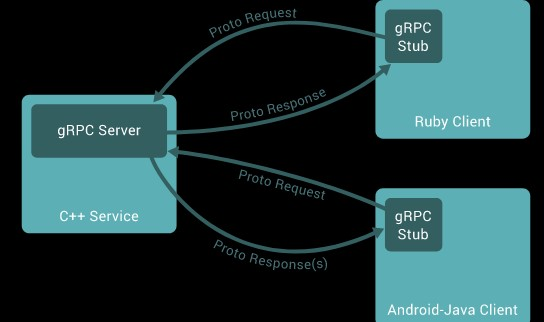
\includegraphics[scale=1]{Figures/6qt1vehe.jpg}
  \caption{نحویه کار \lr{gRPC}}
  \label{Fig:grpc}
  \end{figure}

  
طبق عکس \ref{Fig:grpc}، نحوه کار \lr{gRPC} را با یک سرویس \lr{C++} و کلاینت‌هایی به زبان \lr{Ruby} و \lr{Android-Java} نشان می‌دهد. در اینجا، \lr{gRPC} سرور، مجهز به یک سرویس \lr{C++}، درخواست‌های \lr{Proto} را از کلاینت‌ها دریافت می‌کند و با پاسخ‌های \lr{Proto} پاسخ می‌دهد.

روند ارتباط بین \lr{gRPC} سرور و کلاینت‌ها به شرح زیر است:

هر کلاینت یک \lr{gRPC Stub} را ایجاد می‌کند که یک شیء است که متدهای سرویس را تعریف می‌کند و به آدرس \lr{gRPC} سرور متصل می‌شود.
هر کلاینت یک یا چند درخواست \lr{Proto} را با استفاده از \lr{gRPC Stub} به \lr{gRPC} سرور می‌فرستد. درخواست \lr{Proto} یک پیام است که با پروتوباف تعریف شده است و داده‌های مورد نیاز برای فراخوانی متد سرویس را حاوی است.
\lr{gRPC} سرور درخواست \lr{Proto} را دریافت می‌کند و آن را به متد مربوطه در سرویس \lr{C++} منتقل می‌کند. سرویس \lr{C++} منطق کسب و کار خود را اجرا می‌کند و یک پاسخ \lr{Proto} را تولید می‌کند. پاسخ \lr{Proto} یک پیام است که با پروتوباف تعریف شده است و نتیجه فراخوانی متد سرویس را حاوی است.
\lr{gRPC} سرور پاسخ \lr{Proto} را به \lr{gRPC Stub} کلاینت می‌فرستد. \lr{RPC Stub} پاسخ \lr{Proto} را به زبان کلاینت تبدیل می‌کند و آن را به کلاینت ارائه می‌دهد.

\section{روش های پیشین}

\subsection{استفاده از ماشین های مجازی}
ماشین مجازی یک نرم افزار است که به شما اجازه می دهد یک سیستم عامل دیگر را در داخل سیستم عامل فعلی خود اجرا کنید. برای استفاده از مدل های زبانی بزرگ ها، شما نیاز دارید که یک ماشین مجازی با سیستم عامل ویندوز را نصب کنید و سپس نرم افزار مدل های زبانی بزرگ را در آن اجرا کنید.\cite{tickoo2010modeling} این روش دارای برخی مزایا و معایب است. برخی از مزایای استفاده از ماشین مجازی عبارتند از:
\begin{itemize}[label=-]
  \item
 شما می توانید از مدل های زبانی بزرگ ها بدون نیاز به خرید یک کامپیوتر ویندوز استفاده کنید.
 \item
شما می توانید به راحتی بین سیستم عامل های مختلف جابجا شوید و فایل های خود را به اشتراک بگذارید.
\item
 شما می توانید تنظیمات و پیکربندی های مختلف را برای ماشین مجازی خود انجام دهید و در صورت لزوم به حالت قبل بازگردانید.
\end{itemize}

برخی از معایب استفاده از ماشین مجازی عبارتند از:
\begin{itemize}[label=-]
  \item
   شما نیاز دارید که فضای حافظه و پردازنده کافی را برای اجرای ماشین مجازی فراهم کنید، در غیر این صورت سرعت و عملکرد آن کند خواهد شد.
   \item
    شما نیاز دارید که یک نسخه قانونی از سیستم عامل ویندوز را تهیه و فعال کنید، در غیر این صورت با مشکلات قانونی و امنیتی روبرو خواهید شد.
    \item
     شما نمی توانید از برخی قابلیت های سخت افزاری کامپیوتر خود، مانند دوربین، صدا، چاپگر و غیره، در محیط مجازی استفاده کنید، مگر اینکه درایور های مناسب را نصب کنید.
\end{itemize}

\subsection{مقایسه کانتینرها و ماشین های مجازی}
مقایسه این دو در جدول  \ref{table:msvscon} امده است. که واضح است برای پروژه ما کانتینر ها بهینه تر و مناسب تر هستند.
\begin{table}[!ht]
  \centering
  \caption{مقایسه کانتینرها و ماشین های مجازی}
  \label{table:msvscon}
  \begin{tabular}{l | p{0.35\linewidth} | p{0.6\linewidth}}
  \hline
      ویژگی & ماشین مجازی \lr{(VM)} & کانتینر \\ \hline
      جداسازی & از سیستم عامل میزبان و ماشین‌های مجازی دیگر کاملاً جدا می‌شود. این مورد زمانی مفید است که مرز امنیتی قوی ایجاد شود & از سیستم عامل میزبان و کانتینرهای دیگر به صورت سبک جدا می‌شود، اما مرز امنیتی به اندازه ماشین مجازی قوی نیست \\ \hline
      سیستم عامل & یک سیستم عامل کامل از جمله هسته را اجرا می‌کند و بنابراین منابع سیستم بیشتری (\lr{CPU}، حافظه و ذخیره‌سازی) را مصرف می‌کند & بخش حالت کاربر سیستم عامل را اجرا می‌کند و می‌تواند به گونه‌ای سفارشی شود که فقط خدمات مورد نیاز برنامه را شامل شود \\ \hline
      سازگاری مهمان & می‌تواند هر سیستم عاملی را درون ماشین مجازی اجرا کند & باید با نسخه سیستم عامل میزبان هماهنگ باشد \\ \hline
      مجازی‌سازی & سیستم کامپیوتری را مجازی‌سازی می‌کند، یعنی لایه‌های سخت‌افزاری & سیستم عامل را مجازی‌سازی می‌کند، یعنی فقط لایه‌های نرم‌افزاری \\ \hline
      اندازه & اندازه ماشین مجازی بسیار بزرگ است، معمولاً در مقیاس گیگابایت & اندازه کانتینر بسیار سبک است، معمولاً چند صد مگابایت، اگرچه ممکن است بسته به کاربرد متفاوت باشد \\ \hline
      زمان اجرا & ماشین مجازی زمان بیشتری برای اجرا می‌برد تا کانتینر، زمان دقیق بستگی به سخت‌افزار زیرین دارد & کانتینر زمان خیلی کمتری برای اجرا می‌برد \\ \hline
      حافظه & ماشین مجازی حافظه زیادی را مصرف می‌کند & کانتینر حافظه بسیار کمی را می‌طلبد \\ \hline
      امنیت & ماشین مجازی امن‌تر است، زیرا سخت‌افزار زیرین بین فرآیندها به اشتراک گذاشته نمی‌شود & کانتینر کمتر امن است، زیرا مجازی‌سازی بر پایه نرم‌افزار است و حافظه بین فرآیندها به اشتراک گذاشته می‌شود \\ \hline
      کاربرد & ماشین‌های مجازی زمانی مفید هستند که ما نیاز داریم تمام منابع سیستم عامل را برای اجرای برنامه‌های مختلف استفاده کنیم & کانتینرها زمانی مفید هستند که ما نیاز داریم حداکثر برنامه‌های در حال اجرا را با استفاده از سرورهای حداقلی اجرا کنیم \\ \hline
  \end{tabular}
\end{table}

\begin{figure}[!htb]
  \centering
  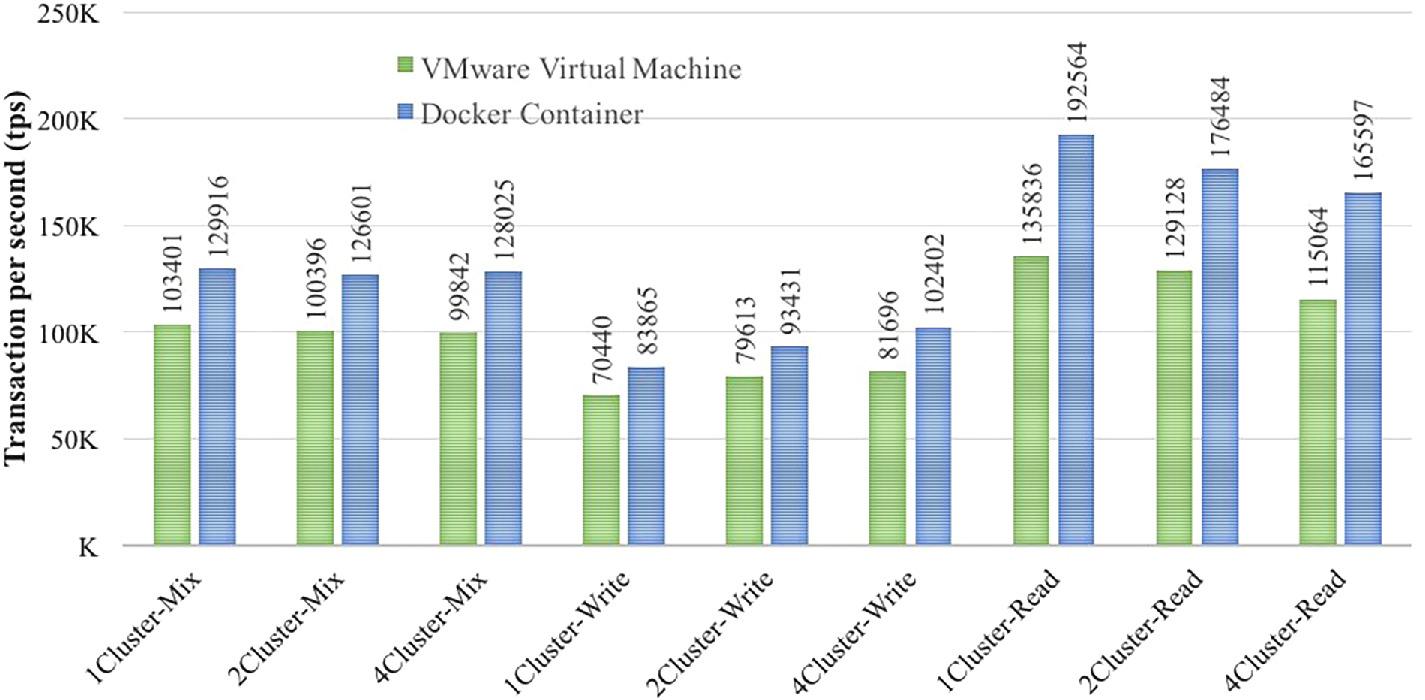
\includegraphics[scale=.16]{Figures/cpe5693-fig-0001-m.jpg}
  \caption{مقایسه استفاده منابع \cite{shirinbab-2020}}
  \end{figure}


\subsection{سرویس های ابری}
سرویس های ابری را می توان برای استفاده از مدل های زبانی بزرگ ها به عنوان یک راه حل مقیاس پذیر و انعطاف پذیر در نظر گرفت. با استفاده از سرویس های ابری، می توان از منابع محاسباتی و ذخیره سازی بدون نگرانی از محدودیت های سخت افزاری بهره برد. همچنین، می توان با استفاده از سرویس های ابری، مدل های زبانی بزرگ ها را به صورت خودکار و پویا مدیریت کرد و به روز رسانی کرد\cite{li2013evaluating}. با این حال، استفاده از سرویس های ابری نیز مشکلات خود را دارد. برخی از مشکلات عبارتند از:
\begin{itemize}[label=-]
  \item
   حفظ امنیت و حریم خصوصی داده ها و مدل های زبانی بزرگ ها در فضای ابری
   \item
   تضمین کیفیت سرویس و عملکرد مناسب مدل های زبانی بزرگ ها در شرایط نامطلوب شبکه
   \item
   هزینه بالای استفاده از سرویس های ابری برای برخی از کاربردهای مدل های زبانی بزرگ ها
   \item
    عدم وجود استانداردهای یکسان و قابل تبادل بین سرویس دهندگان مختلف ابری
\end{itemize}

\begin{table}[!ht]
  \centering
  \caption{هزینه استفاده از سرویس های ابری \lr{Open Ai} \cite{open_ai_pricing_2024}}
  \label{table:pay}
  \begin{tabular}{|l|l|l|}
  \hline
      \lr{Model} & \lr{Input} & \lr{Output} \\ \hline
      \lr{gpt-4} & \lr{\$0.03/ 1K tokens} & \lr{\$0.06/ 1K tokens} \\ \hline
      \lr{gpt-4-32k} & \lr{\$0.06/ 1K tokens} & \lr{\$0.12/ 1K tokens} \\ \hline
  \end{tabular}
\end{table}

با توجه به جدول \ref{table:pay} برای تولید 1000 توکن شما باید حدود \lr{58 \$} پرداخت کنید.

\begin{figure}[!htb]
  \centering
  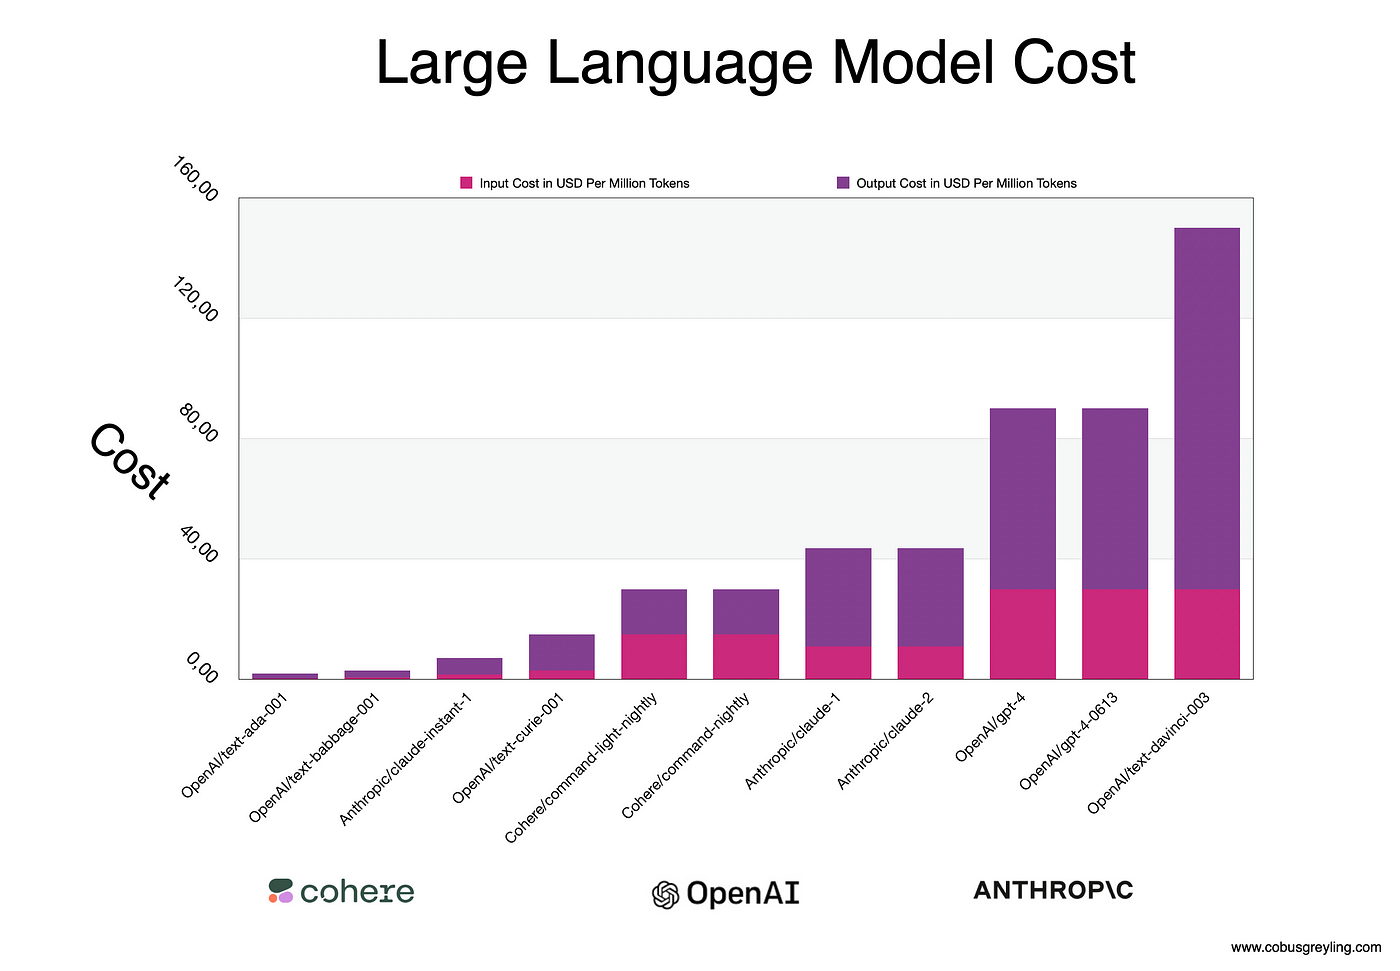
\includegraphics[scale=.3]{Figures/657b748bc22e00d9d57ba827_6502a4b5bada5953b9d8aff6_1 FWRHD8OaVBAF-yNhpT2fOQ.png}
  \caption{مقایسه هزینه ها برای اسفاده از سرویس های ابری\cite{greyling}}
\end{figure}

\subsection{استفاده مستقیم از مدل های زبانی بزرگ}
برای استفاده مستقیم از مدل های زبانی بزرگ نیاز مشکلات زیر را به همراه دارد
\begin{itemize}[label=-]
  \item
   نیاز به فرد متخصص
   \item
   عدم مقیاس پذیری
   \item
  امکان استفاده ان در سیستم عامل ها مختلف وجود ندارد
\end{itemize}

\section{روش پیشنهادی}
\subsection{استفاده از کانتینر ها}

کانتنر ها راهی برای بسته بندی و اجرای برنامه های کامپیوتری هستند که می توانند در محیط های مختلف اجرا شوند. کانتنر ها مزایایی مانند سادگی، قابلیت حمل و نقل، امنیت و کارایی دارند. برای انتشار مدل های زبانی بزرگ، کانتنر ها می توانند راه حل مناسبی باشند. چون:
\begin{itemize}[label=-]
  \item
   کانتنر ها می توانند مدل ها را به صورت جداگانه و مستقل از سخت افزار و سیستم عامل اجرا کنند. این به این معنی است که مدل ها را نیازی نیست برای هر پلتفرم یا دستگاه جدید تغییر داد یا تطبیق داد.
   \item
   کانتنر ها می توانند مدل ها را به صورت خودکار و پویا مقیاس بزرگ کنند. این به این معنی است که بر اساس نیاز و تقاضای کاربران، تعداد و منابع کانتنر ها را می توان افزایش یا کاهش داد.
   \item
   کانتنر ها می توانند مدل ها را به صورت امن و قابل اعتماد اجرا کنند. این به این معنی است که کانتنر ها محافظت شده از دسترسی های غیرمجاز یا خطای سخت افزار یا نرم افزار هستند.
\end{itemize}
برای استفاده از کانتنر ها برای انتشار مدل های زبانی بزرگ، لازم است چند قدم را طی کنیم:
\begin{itemize}[label=-]
  \item
   ابتدا باید یک تصویر \LTRfootnote{image} کانتنر را بسازید. تصویر کانتنر شامل کدهای، پکیج های، پیکربندی های و داده های لازم برای اجرای مدل است.
   \item
   سپس باید تصویر کانتنر را در یک رجیستر \LTRfootnote{registry} آپلود کنید. رجیستر یک سرویس ذخیره سازی است که تصویر کانتنر را در دسترس قرار می دهد.
   \item
   در نهایت باید یک نمونه \LTRfootnote{instance} از تصویر کانتنر را در یک سرویس حمل و نقل \LTRfootnote{transport} درخواست کنید. سرویس حمل و نقل چگونگی و کجای اجرای نمونه را تعیین می کند.
\end{itemize}
ولی این مراحل دسترسی سریع را برای کاربر اینجا نمی کند. چون همچنان کار با این نوع سیستم ساخته شده مشکل است.

\subsection{مدیریت کانتنر های ساخته شده برای مدل های زبانی بزرگ}
\begin{itemize}[label=-]
  \item
  برای اجرای مدل مدل ﻫﺎﻱ ﺯﺑﺎﻧﻲ ﺑﺰﺭگ ، ما از فناوری کانتینر استفاده می‌کنیم که با استانداردهای \lr{Open Container Initiative} \cite{girma2018evaluation} سازگار است. این فناوری به ما امکان می‌دهد که مدل را به صورت جدا و مستقل از سیستم عامل و محیط اجرایی بسته‌بندی و اجرا کنیم.
  \item
  برای اجرای کانتینر مدل مدل ﻫﺎﻱ ﺯﺑﺎﻧﻲ ﺑﺰﺭگ ، ما از یک اجراکننده کانتینر به نام \lr{youki} \cite{containers/youki_2024} استفاده می‌کنیم که یک پیاده‌سازی کامل از استاندارد \lr{OCI} است. این اجراکننده کانتینر به ما امکان می‌دهد که کانتینر را با سرعت و امنیت بالا اجرا کنیم.
  \item
  برای تنظیم وابستگی‌های مورد نیاز مدل مدل ﻫﺎﻱ ﺯﺑﺎﻧﻲ ﺑﺰﺭگ ، ما یک فایل تنظیمات به فرمت \lr{JSON} ایجاد می‌کنیم که شامل اطلاعاتی مانند نام کانتینر، نسخه مدل، پارامترهای مدل، حافظه مورد نیاز، پورت‌های مورد استفاده و دیگر تنظیمات مربوطه است. این فایل تنظیمات به اجراکننده کانتینر ارسال می‌شود تا کانتینر را با توجه به آن ایجاد و اجرا کند.
  \item
  برای ارتباط با مدل مدل ﻫﺎﻱ ﺯﺑﺎﻧﻲ ﺑﺰﺭگ ، ما از دو پروتوکل و \lr{gRPC}  پشتیبانی می‌کنیم. پروتوکل \lr{HTTP}  یک پروتوکل مبتنی بر درخواست-پاسخ است که از طریق وب ارتباط برقرار می‌کند. پروتوکل \lr{gRPC} یک پروتوکل مبتنی بر \lr{RPC} است که از طریق پروتوکل \lr{HTTP/2} ارتباط برقرار می‌کند. این دو پروتوکل به ما امکان می‌دهند که با استفاده از فرمت‌های مختلفی مانند \lr{JSON}، \lr{XML}، \lr{Protobuf} \cite{popic2016performance} و غیره، داده‌ها را به مدل ارسال و از مدل دریافت کنیم. برای تنظیم پروتوکل‌ها و تنظیمات مربوطه، ما از فایل‌های تعریف سرویس و تنظیمات استفاده می‌کنیم که شامل اطلاعاتی مانند نام سرویس، نوع درخواست، نوع پاسخ، پورت‌ها، مسیرها و دیگر جزئیات مربوطه است. این فایل‌ها به اجراکننده کانتینر ارسال می‌شوند تا پروتوکل‌ها و تنظیمات را برای کانتینر فعال کند.
  \item و برای کاربران عادی نیز که نیاز به \lr{ََAPI} \cite{bloch2006design} ندارند یک صفحه وب تهیه می شود که می توانند با ان به راحتی با مدلی که نصب کرده اند ارتباط برقرار کنند.
\end{itemize}

\subsection{چرا این روش برای کاربران عادی بهتر است؟}
استفاده از کانتینرها برای اجرای سریع و محلی مدل‌های زبانی بزرگ می‌تواند برای یک کاربر عادی مفید باشد، زیرا:
\begin{itemize}
  \item 

کانتینرها از منابع سیستم کمتری نسبت به ماشین‌های مجازی استفاده می‌کنند و بنابراین می‌توانند سرعت و کارایی بالاتری داشته باشند.
  \item 

کانتینرها امکان اجرای مدل‌های زبانی بر روی \lr{CPU} را فراهم می‌کنند، که ممکن است برای کاربرانی که \lr{GPU} ندارند یا محدودیت‌های هزینه‌ای دارند مفید باشد.
\item 

کانتینرها امکان اجرای مدل‌های زبانی بدون نیاز به اتصال به اینترنت را می‌دهند، که می‌تواند برای حفظ حریم خصوصی و امنیت کاربران مهم باشد.
\item 

کانتینرها امکان انتخاب و تغییر مدل‌های زبانی را به راحتی فراهم می‌کنند، که می‌تواند برای انجام وظایف مختلف و تنظیم پارامترهای مدل مفید باشد.
\end{itemize}

\subsection{چرا این روش برای شرکت ها بهتر است؟}
مزایای استفاده از کانتینرها برای شرکت ها:
\begin{itemize}
\item 
کاهش هزینه‌ها: با استفاده از کانتینرها، می‌توان مدل‌های زبانی بزرگ را بر روی سخت‌افزارهای محلی اجرا کرد، بدون نیاز به استفاده از سرویس‌های ابری یا اینترنت. این کار می‌تواند هزینه‌های مربوط به پردازش، ذخیره‌سازی و انتقال داده‌ها را کاهش دهد.
\item 
افزایش امنیت: با استفاده از کانتینرها، می‌توان مدل‌های زبانی بزرگ را در محیط‌های ایزوله و کنترل شده اجرا کرد، بدون نیاز به اشتراک‌گذاری داده‌ها یا مدل‌ها با سرویس‌های خارجی. این کار می‌تواند خطرات مربوط به نشت اطلاعات، سوءاستفاده از مدل‌ها یا حملات سایبری را کاهش دهد.
\item 
افزایش سرعت: با استفاده از کانتینرها، می‌توان مدل‌های زبانی بزرگ را با زمان راه‌اندازی کمتر و بازدهی بالاتر اجرا کرد، به دلیل بسته‌بندی قبلی برنامه‌ها و وابستگی‌ها. این کار می‌تواند تجربه کاربری را سریع‌تر و پاسخگوتر کند.
\item 
افزایش مقیاس‌پذیری: با استفاده از کانتینرها، می‌توان مدل‌های زبانی بزرگ را به راحتی بر اساس تقاضا بزرگنمایی یا کوچکنمایی کرد.
\end{itemize}
% !TEX root = ../ui-thesis.tex
% !TeX program = xelatex

\chapter{نتیجه‌گیری و پیشنهادها}
\section{‌نتیجه‌گیری}
نوشته نمونه نوشته نمونه نوشته نمونه نوشته نمونه نوشته نمونه نوشته نمونه نوشته نمونه نوشته نمونه نوشته نمونه نوشته نمونه نوشته نمونه نوشته نمونه نوشته نمونه نوشته نمونه نوشته نمونه نوشته نمونه نوشته نمونه نوشته نمونه نوشته نمونه نوشته نمونه نوشته نمونه نوشته نمونه. نوشته نمونه نوشته نمونه نوشته نمونه نوشته نمونه نوشته نمونه نوشته نمونه نوشته نمونه نوشته نمونه نوشته نمونه نوشته نمونه نوشته نمونه نوشته نمونه نوشته نمونه نوشته نمونه نوشته نمونه نوشته نمونه نوشته نمونه نوشته نمونه نوشته نمونه نوشته نمونه نوشته نمونه نوشته نمونه. نوشته نمونه نوشته نمونه نوشته نمونه نوشته نمونه نوشته نمونه نوشته نمونه نوشته نمونه نوشته نمونه نوشته نمونه نوشته نمونه نوشته نمونه نوشته نمونه نوشته نمونه نوشته نمونه نوشته نمونه نوشته نمونه نوشته نمونه نوشته نمونه نوشته نمونه نوشته نمونه نوشته نمونه نوشته نمونه. نوشته نمونه نوشته نمونه نوشته نمونه نوشته نمونه نوشته نمونه نوشته نمونه نوشته نمونه نوشته نمونه نوشته نمونه نوشته نمونه نوشته نمونه نوشته نمونه نوشته نمونه نوشته نمونه نوشته نمونه نوشته نمونه نوشته نمونه نوشته نمونه نوشته نمونه نوشته نمونه نوشته نمونه نوشته نمونه. نوشته نمونه نوشته نمونه نوشته نمونه نوشته نمونه نوشته نمونه نوشته نمونه نوشته نمونه نوشته نمونه نوشته نمونه نوشته نمونه نوشته نمونه نوشته نمونه نوشته نمونه نوشته نمونه نوشته نمونه نوشته نمونه نوشته نمونه نوشته نمونه نوشته نمونه نوشته نمونه نوشته نمونه نوشته نمونه. نوشته نمونه نوشته نمونه نوشته نمونه نوشته نمونه نوشته نمونه نوشته نمونه نوشته نمونه نوشته نمونه نوشته نمونه نوشته نمونه نوشته نمونه نوشته نمونه نوشته نمونه نوشته نمونه نوشته نمونه نوشته نمونه نوشته نمونه نوشته نمونه نوشته نمونه نوشته نمونه نوشته نمونه نوشته نمونه. نوشته نمونه نوشته نمونه نوشته نمونه نوشته نمونه نوشته نمونه نوشته نمونه نوشته نمونه نوشته نمونه نوشته نمونه نوشته نمونه نوشته نمونه نوشته نمونه نوشته نمونه نوشته نمونه نوشته نمونه نوشته نمونه نوشته نمونه نوشته نمونه نوشته نمونه نوشته نمونه نوشته نمونه نوشته نمونه.

\section{پیشنهادها}
نوشته نمونه نوشته نمونه نوشته نمونه نوشته نمونه نوشته نمونه نوشته نمونه نوشته نمونه نوشته نمونه نوشته نمونه نوشته نمونه نوشته نمونه نوشته نمونه نوشته نمونه نوشته نمونه نوشته نمونه نوشته نمونه نوشته نمونه نوشته نمونه نوشته نمونه نوشته نمونه نوشته نمونه نوشته نمونه. نوشته نمونه نوشته نمونه نوشته نمونه نوشته نمونه نوشته نمونه نوشته نمونه نوشته نمونه نوشته نمونه نوشته نمونه نوشته نمونه نوشته نمونه نوشته نمونه نوشته نمونه نوشته نمونه نوشته نمونه نوشته نمونه نوشته نمونه نوشته نمونه نوشته نمونه نوشته نمونه نوشته نمونه نوشته نمونه. نوشته نمونه نوشته نمونه نوشته نمونه نوشته نمونه نوشته نمونه نوشته نمونه نوشته نمونه نوشته نمونه نوشته نمونه نوشته نمونه نوشته نمونه نوشته نمونه نوشته نمونه نوشته نمونه نوشته نمونه نوشته نمونه نوشته نمونه نوشته نمونه نوشته نمونه نوشته نمونه نوشته نمونه نوشته نمونه. نوشته نمونه نوشته نمونه نوشته نمونه نوشته نمونه نوشته نمونه نوشته نمونه نوشته نمونه نوشته نمونه نوشته نمونه نوشته نمونه نوشته نمونه نوشته نمونه نوشته نمونه نوشته نمونه نوشته نمونه نوشته نمونه نوشته نمونه نوشته نمونه نوشته نمونه نوشته نمونه نوشته نمونه نوشته نمونه. نوشته نمونه نوشته نمونه نوشته نمونه نوشته نمونه نوشته نمونه نوشته نمونه نوشته نمونه نوشته نمونه نوشته نمونه نوشته نمونه نوشته نمونه نوشته نمونه نوشته نمونه نوشته نمونه نوشته نمونه نوشته نمونه نوشته نمونه نوشته نمونه نوشته نمونه نوشته نمونه نوشته نمونه نوشته نمونه. نوشته نمونه نوشته نمونه نوشته نمونه نوشته نمونه نوشته نمونه نوشته نمونه نوشته نمونه نوشته نمونه نوشته نمونه نوشته نمونه نوشته نمونه نوشته نمونه نوشته نمونه نوشته نمونه نوشته نمونه نوشته نمونه نوشته نمونه نوشته نمونه نوشته نمونه نوشته نمونه نوشته نمونه نوشته نمونه. نوشته نمونه نوشته نمونه نوشته نمونه نوشته نمونه نوشته نمونه نوشته نمونه نوشته نمونه نوشته نمونه نوشته نمونه نوشته نمونه نوشته نمونه نوشته نمونه نوشته نمونه نوشته نمونه نوشته نمونه نوشته نمونه نوشته نمونه نوشته نمونه نوشته نمونه نوشته نمونه نوشته نمونه نوشته نمونه.


% ░░░░░░░▒▒▒▒▒▒▓▓▓▓ References ▓▓▓▓▒▒▒▒▒▒░░░░░░░
% References.bib نام فایل حاوی رفرنس‌ها است.
\MakeReferences{References}

% ----------------------------------------------------------------------------
%\clearpage
\pagestyle{myheadings}
%\pagenumbering{arabic}
%\setcounter{page}{1}

% ░░░░░░░▒▒▒▒▒▒▓▓▓▓ Chapters ▓▓▓▓▒▒▒▒▒▒░░░░░░░
%\clearpage
%\baselineskip=0.9cm
\linespread{1.0} % single-line spacing
%\linespread{1.3} % one and a half line spacing
%\linespread{1.6} % double-line spacing


\settextfont[Scale=1.2, ItalicFont=*, ItalicFeatures={FakeSlant=0.32}, BoldItalicFont=* Bold, BoldItalicFeatures={FakeSlant=0.32}]{B Nazanin}
\titleformat{\chapter}[display]
{\fontsize{15pt}{0}\selectfont  \flushleft  \bfseries \BNazaninScaleOne} % B Nazanin 15
{\chaptertitlename\ \tartibi{chapter}}{0.3cm}{\fontsize{15pt}{0}\selectfont \BNazaninScaleOne} % B Nazanin 15
\sectionfont{\fontsize{14pt}{\baselineskip}\selectfont \bfseries \BNazaninScaleOne} % B Nazanin 14
\subsectionfont{\fontsize{13pt}{\baselineskip}\selectfont \bfseries \BNazaninScaleOne} % B Nazanin 13
\subsubsectionfont{\fontsize{13pt}{\baselineskip}\selectfont \bfseries \BNazaninScaleOne} % B Nazanin 13

%\titlespacing*{\chapter}{0pt}{3.5cm}{8cm}
\titlespacing*{\section}{0pt}{1.2\baselineskip}{0pt}
\titlespacing*{\subsection}{0pt}{1.1\baselineskip}{0pt}
\titlespacing*{\subsubsection}{0pt}{1\baselineskip}{0pt}

\makeatletter
\renewcommand\chapter{\if@openright\cleardoublepage\else\clearpage\fi
	%\thispagestyle{empty}
	\global\@topnum\z@
	\@afterindentfalse
	\secdef\@chapter\@schapter}
\makeatother

% ░░░░░░░▒▒▒▒▒▒▓▓▓▓ Appendices ▓▓▓▓▒▒▒▒▒▒░░░░░░░
%\addtocontents{lof}{\protect\setcounter{tocdepth}{0}} % ignore adding appendix figures to list of figures
%\addtocontents{lot}{\protect\setcounter{tocdepth}{0}} % ignore adding appendix table to list of tables
\captionsetup{list=no}

\end{document} 

